\section{Background}
\label{sec:preliminary}



\begin{figure*}[t]
\centering
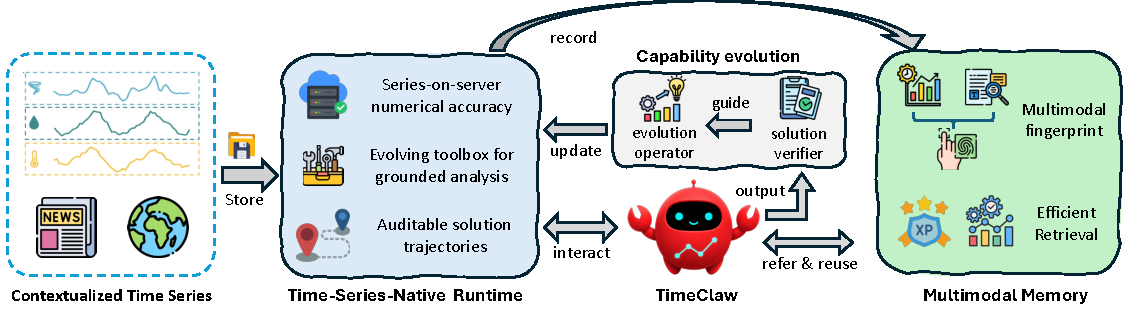
\includegraphics[width=\linewidth]{figures/framework.pdf}
\caption{
Overview of \method. 
Given contextualized time series, \method operates through a time-series-native runtime that provides server-side numerical execution, an evolving toolbox for grounded analysis, and auditable solution trajectories (Section \ref{sec:tools}).
The agent further improves over time through capability evolution (Section \ref{sec:evolve}) and retrieves relevant experience from multimodal memory via multimodal fingerprints (Section \ref{sec:memory}).
}
\label{fig:main}
\vspace{-3mm}
\end{figure*}



\subsection{Preliminary}

We use calligraphic letters (e.g., $\mathcal{A}$) for sets and bold capital letters for matrices (e.g., $\bm{A}$). For matrix indices, $\bm{A}[i, j]$ denotes the entry in the $i^{\textrm{th}}$ row and the $j^{\textrm{th}}$ column. For a vector $\bm{v}$, $v[i:j]$ represents the sub-vector sliced from the $i^{\textrm{th}}$ to the $j^{\textrm{th}}$ position, inclusively. $\bm{A}[i, :]$ returns the $i^{th}$ row in $\bm{A}$ and $\bm{A}[:i]$ returns the first $i$ rows of $\bm{A}$.

\paragraph{Time Series and Contextualized Time Series.} A \textit{numerical time series} is denoted as
\begin{equation}
    \mathbf{X}_{1:T} = [\mathbf{x}_1, \mathbf{x}_2, \ldots, \mathbf{x}_T] \in \mathbb{R}^{N \times T},
\end{equation}
where $T$ is the number of timestamps, $N$ is the number of variables, and $\mathbf{x}_t \in \mathbb{R}^{N}$ is the observation at timestamp $t$. For $1 \leq a \leq b \leq T$, we denote the temporal slice from timestamp $a$ to $b$ as
\begin{equation}
    \mathbf{X}_{a:b}
    =
    [\mathbf{x}_a, \mathbf{x}_{a+1}, \ldots, \mathbf{x}_b].
\end{equation}
We define a \textit{contextualized time series} as
\begin{equation}
    \mathcal{X}
    =
    (\mathbf{X}_{1:T}, \mathcal{C}),
\end{equation}
where $\mathbf{X}_{1:T}$ is the numerical temporal signal and $\mathcal{C}$ is the associated context. The context $\mathcal{C}$ may contain information from various sources, such as textual descriptions, categorical metadata, external constraints, and domain knowledge. In this work, we focus on the text-time series mixture, a special case of contextualized time series. This setting is broadly representative of many real-world temporal reasoning scenarios where textual cues provide essential information for interpreting temporal dynamics and supporting decisions. Yet the core methodology is generalizable across additional context sources beyond natural language.
\paragraph{From Predefined Tasks to Open-Ended Temporal Reasoning.} Conventional time-series learning is usually defined by fixed task mappings, such as $\mathbf{X}_{1:T} \mapsto \mathbf{X}_{T+1:T+H}$ for forecasting or $\mathbf{X}_{1:T} \mapsto y$ for classification. We define \textit{open-ended contextualized temporal reasoning} as a more general setting where the task objective and output format are specified by a natural-language instruction, and the numerical time series is interpreted together with its associated context. Given a contextualized time series
$\mathcal{X}=(\mathbf{X}_{1:T},\mathcal{C})$, we define a task instance as
\begin{equation}
    \tau = (q, \mathcal{X}, \mathcal{Y}, y^\star, \ell),
\end{equation}
where $q$ is the instruction, $\mathcal{Y}$ is the output space, $y^\star \in
\mathcal{Y}$ is the target, and $\ell:\mathcal{Y}\times\mathcal{Y}\to\mathbb{R}$
is the evaluation function. The goal is to produce
\begin{equation}
    \hat{y}=f(q,\mathcal{X})\in\arg\min_{y\in\mathcal{Y}}\ell(y,y^\star).
\end{equation}
Here $\mathcal{Y}$ may include numerical predictions, labels, rankings, textual
explanations, decisions, executable actions, or their combinations. 



\subsection{Why NOT Fully Trust LLMs?}
\textbf{LLM Workflow for Time Series.}
Existing LLM-based agents usually process contextualized time series through
textual serialization. Given $\mathcal{X}=(\mathbf{X}_{1:T},\mathcal{C})$, a
serialization function $\sigma$ maps the numerical series and context to text
$s_\mathcal{X}=\sigma(\mathcal{X})$. The LLM then tokenizes the instruction and serialized input as
\begin{equation}
    \mathbf{z}_{1:L}=\operatorname{Tokenize}([q;s_{\mathcal{X}}]),
\end{equation}
\textbf{Limitations.}
This text-centric workflow introduces two forms of misalignment. First,
\textit{data-type misalignment} arises because numerical temporal signals are
converted into discrete text tokens. As a result, numerical proximity, temporal
resolution, long-range dependencies, and fine-grained variations may not be
faithfully preserved under tokenization and finite context budgets. Second,
\textit{agentic-process misalignment} arises because the agent reasons over
serialized text rather than native temporal objects. Operations that are natural
for time series, such as slicing, aggregation, decomposition, smoothing,
forecasting, anomaly localization, and numerical verification, become indirect
language-based reasoning steps. Due to page limitations, we provide a more detailed analysis of these
limitations in Appendix~\ref{ap:analysis}, including numerical-token
distance mismatch, decimal place-value distortion, next-token versus next-value
objective mismatch, and long-context temporal information dilution. 